\section{Switchless Architecture}
\label{sec:arch}

The switchless architecture, as the name implies, removes switches from the data center network architecture.  Instead, switches are integrated into servers and the topology is chosen to keep the fanout of the in-server switches low.  The in-server switches could be implemented as separate boards attach to the server's I/O bus or they could be directly integrated with the processor on die.  We choose to focus on integrating the switches with the processor on die since silicon area is cheap and the latency from the processor to the switch is lower (and we are computer architects!).  In the following subsections, we discuss switchless network topologies, the design of in-server switches, the switchless network stack, and the benefits that come with the switchless architecture.

\subsection{Switchless Network Topologies}

We focus on two switchless network topologies, torus and cube.  The torus topology, Figure~\ref{fig:switchless_arch_torus}, is a two-dimensional topology where nodes are placed in a two-dimensional grid and are connected in all directions (north, south, east, and west).  Nodes at the edges have links that wrap around to the node at the opposite edge.  This creates a mesh fabric of nodes.  The cube topology, Figure~\ref{fig:switchless_arch_cube}, is similar to the torus topology with one additional dimension.  Nodes are placed into a three-dimensional grid and are also connected in all directions.  The cube topology with the same number of nodes as a given torus topology has higher bandwidth and lower average latency since nodes have more neighbors and the maximum hop count is lower.  Both of these topology limit the fanout of the in-server switch to four or six ports.

One consideration when designing a data center network topology is wiring complexity.  While complex wiring is not a fundamental problem, it can affect the time and cost to setup the data center as well as the link length.  There is a tradeoff between bandwidth and cost of a link when considering link length.  Longer links are required to either be lower bandwidth or require a different link.  The bandwidth requirement of long links can be met by using thicker cabling or different cable technologies, such as optical links.  These links, however, are more expensive.

The cube topology actually maps well to a data center as far as wiring goes.  If racks are arranged in a two-dimensional grid, you can think of each layer of nodes in the racks as a torus.  A cube can be created by connecting the tori vertically.  Thus, the wiring is rather trivial.  A torus topology does not map as well to the data center, so the wiring may be more complex.  However, as mentioned earlier, this problem is not fundamental and can be solved.

\begin{figure}
    \centering
    \subfloat[Torus]
    {
        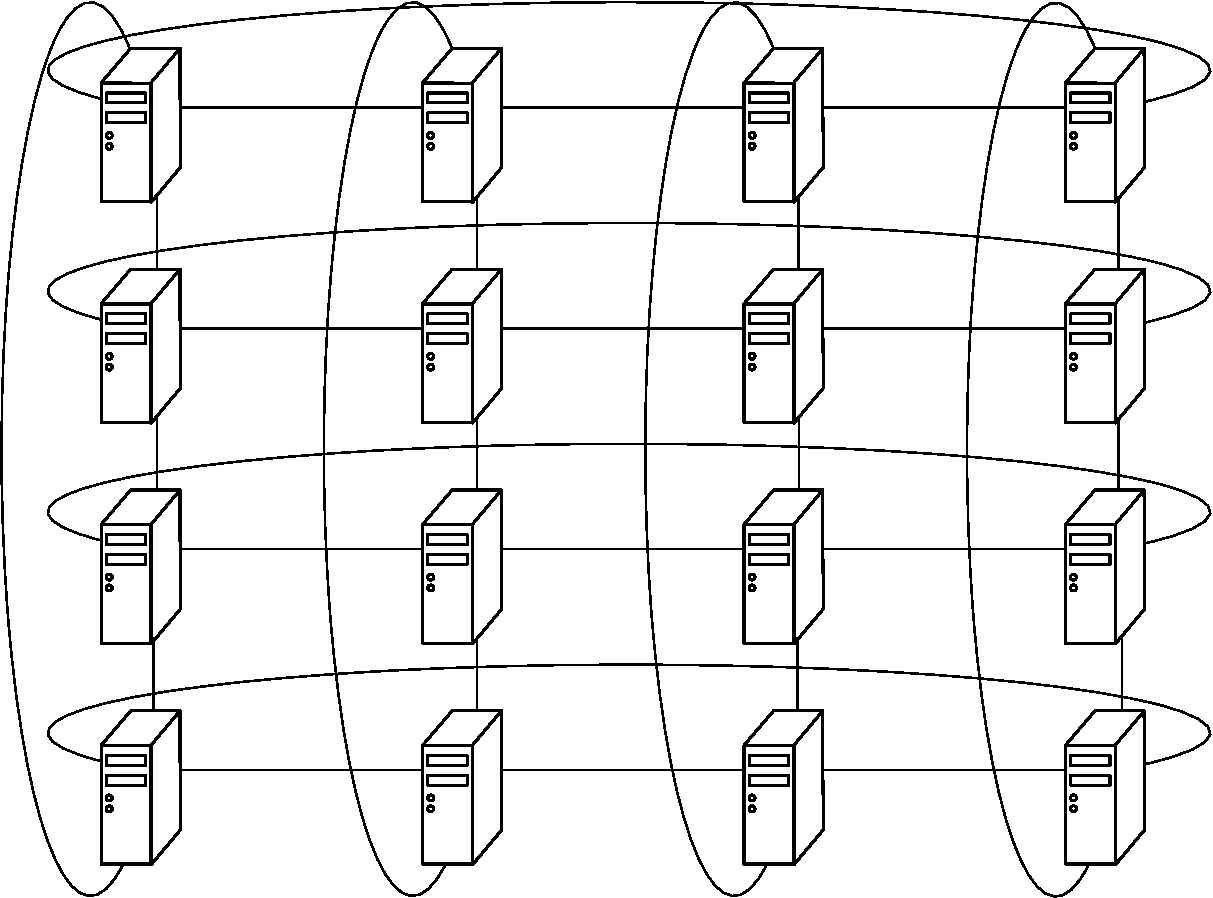
\includegraphics[width=0.2\textwidth]{switchless-arch-torus}
        \label{fig:switchless_arch_torus}
    }
    \\
    \vspace{-0.05in}
    \subfloat[Cube]
    {
        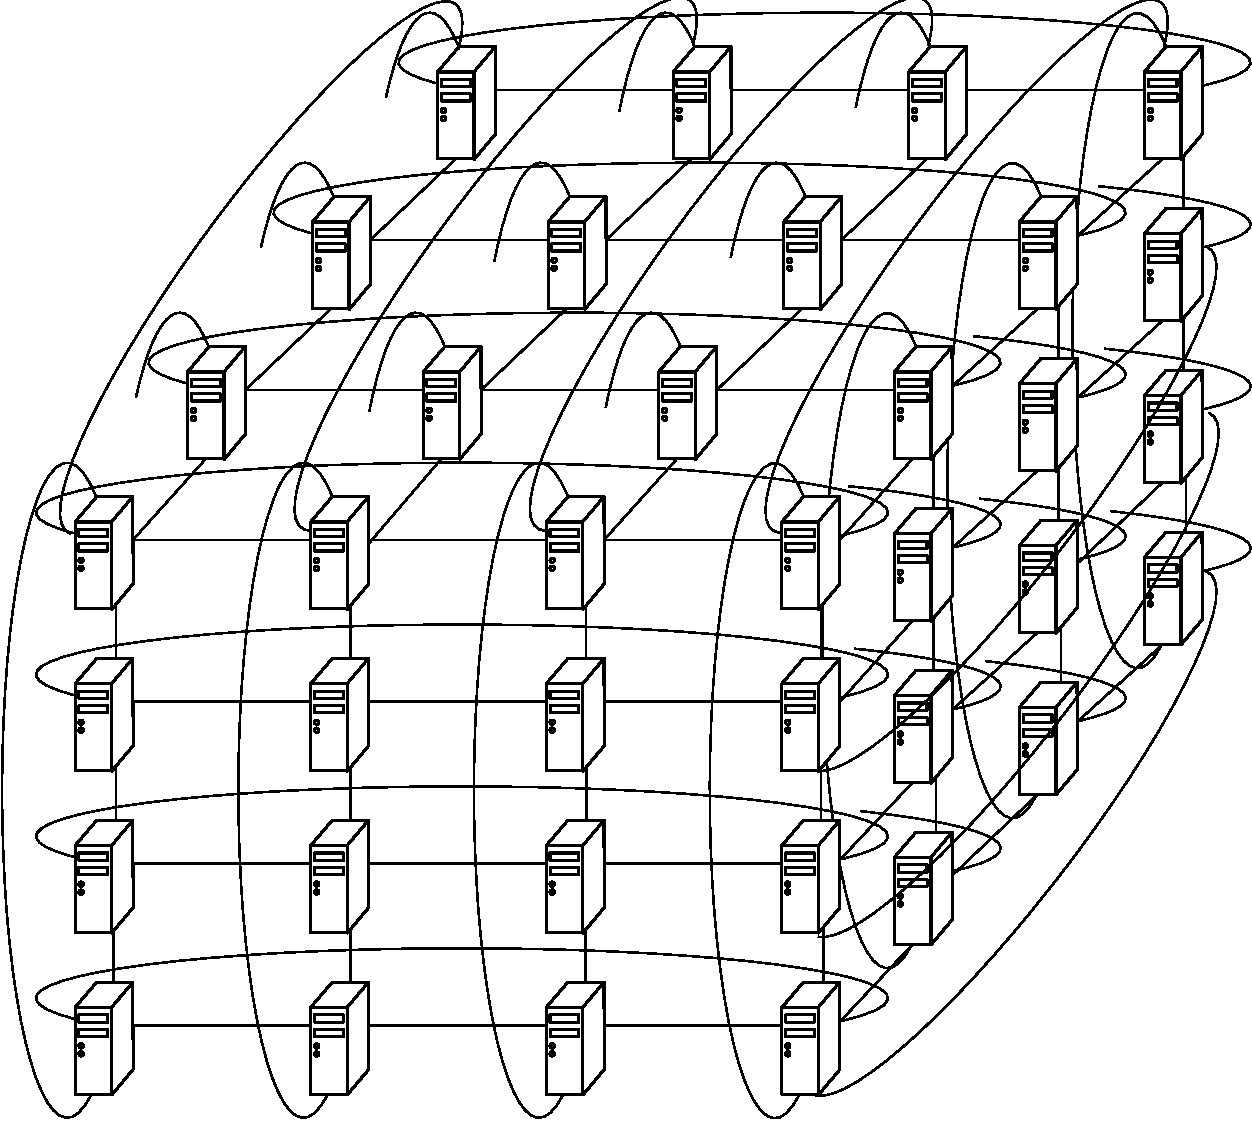
\includegraphics[width=0.25\textwidth]{switchless-arch-cube}
        \label{fig:switchless_arch_cube}
    }
    \vspace{-0.07in}
    \caption{Switchless Data Center Network Topologies}
    \label{fig:switchless_topos}
\end{figure}

\subsection{In-Server Switch Design}

We focus on integrating the switch with the processor on die.  As was mentioned previously, this is beneficial because silicon area is cheap and the latency from the processor to the switch is lower.  The switch can be connected to the processor through the I/O bus or the network on chip (or any other interconnect architecture), as shown in Figure~\ref{fig:in_server_switch_design}.  In either case, the processor and switch can communicate through memory-mapped I/O.  

As for the in-server switch itself, it can be implemented either as custom logic or a general-purpose dedicated core.  Custom logic, which essentially acts as an accelerator, is higher performance and more energy efficient, however, a general-purpose dedicated core is more simple and flexible.  A general-purpose dedicated core may also be more desirable for software defined networks (SDN), where the routing protocol can be configured based on the application and network conditions.  Both designs are acceptable and there is no defining factor which makes one superior to the other.

\begin{figure}
    \centering
    \subfloat[Bus Based Design]
    {
        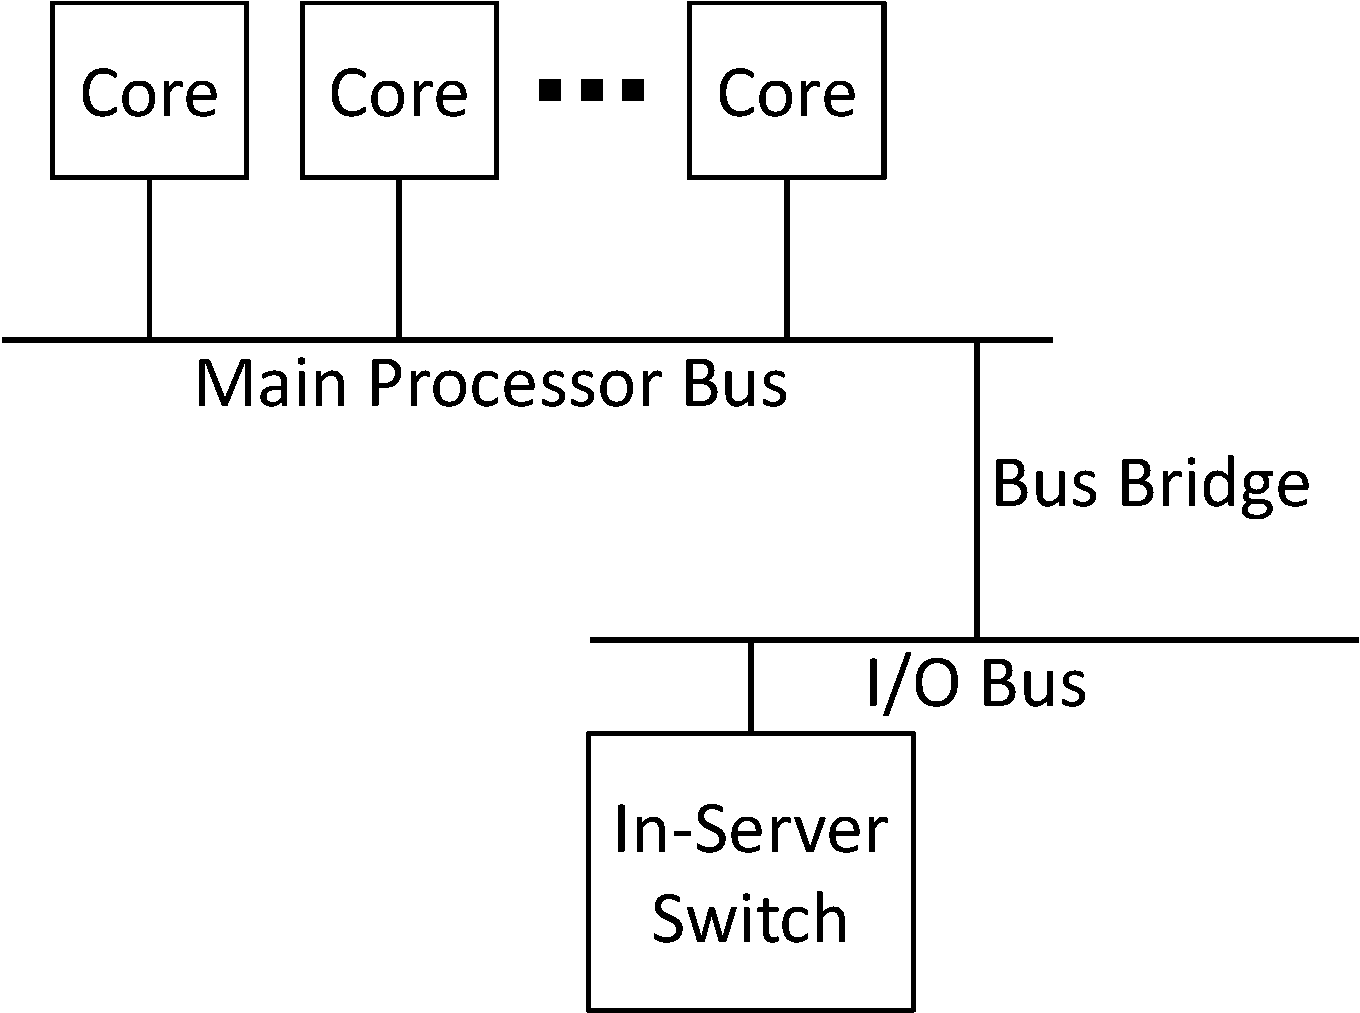
\includegraphics[width=0.2\textwidth]{in-server-switch-bus}
        \label{fig:in_server_bus}
    }
    ~
    \subfloat[Network on Chip Design]
    {
        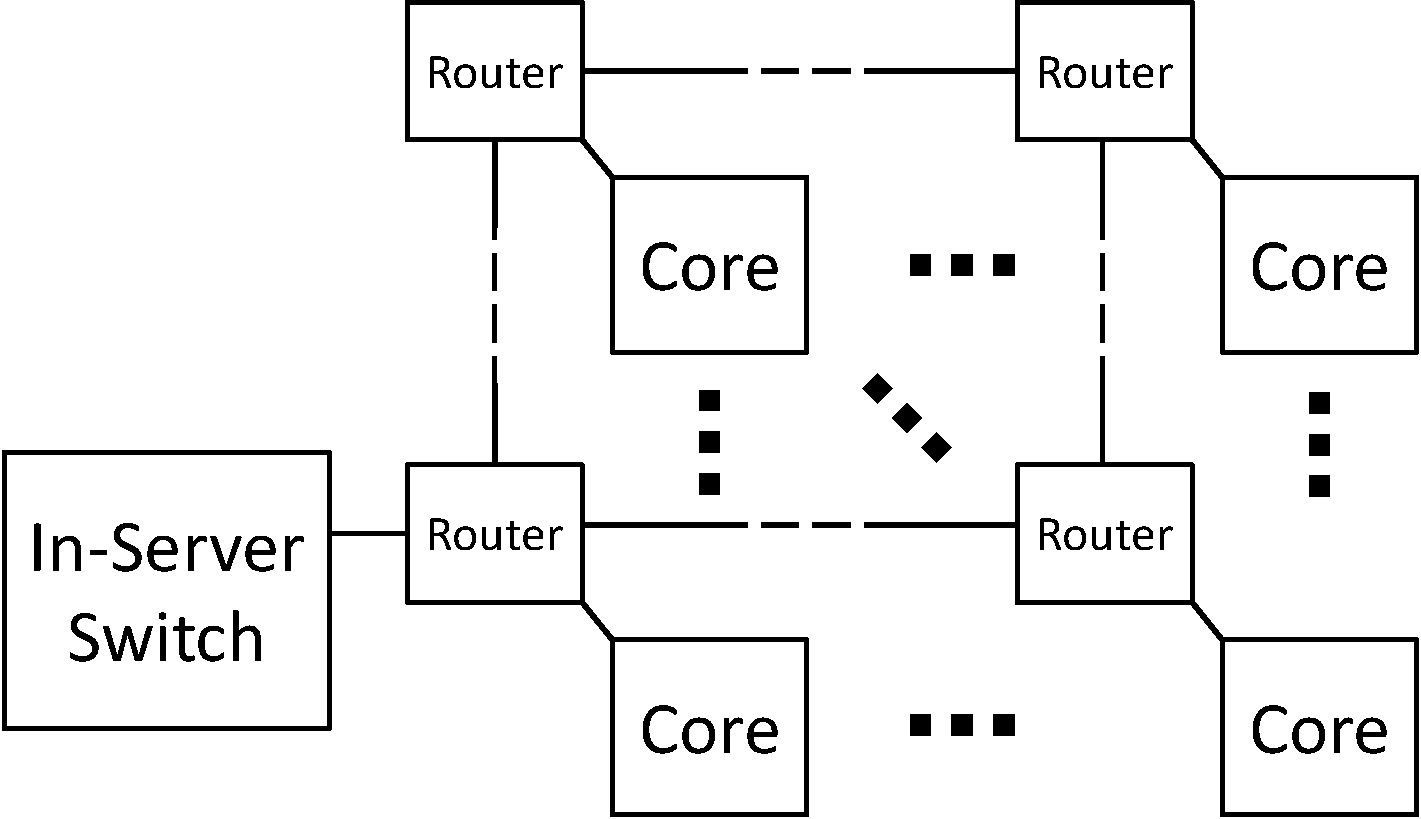
\includegraphics[width=0.2\textwidth]{in-server-switch-noc}
        \label{fig:in_server_noc}
    }
    \vspace{-0.07in}
    \caption{In-Server Switch Processor Integration}
    \label{fig:in_server_switch_design}
\end{figure}

\subsection{Switchless Network Stack}

The switchless network topologies enable the use of a simpler network protocol stack.  We believe that IP is rather heavyweight for internal routing in a data center, especially for statically configured geometrical topologies like the switchless topologies we consider.  Thus, we propose using dimension ordered routing~\cite{Ni:1993:SWRTDN} for the torus and cube topologies.  In dimension ordered routing, all nodes are assigned an address, generally based on the location within the topology (i.e. (X, Y, Z) for cube), and is statically configured with this address.  Thus, a switch knows that sending out one interface increases in the X direction and sending out another interface decreases in the X direction.  The same is true for all dimensions.  Which interfaces point in which direction must be statically configured.  

When a switch receives a packet, it simply compares the destination address to its assigned address and can determine whether the packet is destined for the local node or must be forwarded out an interface which advances it towards the destination node.  The interface to forward a packet over can be determined by comparing the destination address dimensions with the local address dimensions.  In dimension ordered routing, dimensions are given priority.  For example, route in the X direction until it reaches the correct X position, then route in the Y direction, then the Z direction.

This protocol is much more lightweight than IP, and does not require the address resolution protocol (ARP) in order to function (which is also heavyweight, requiring lots of communication).  Routing decisions can be made quicker and the paths packets take will be no longer than the paths IP would choose.  The protocol could also be improved to do adaptive routing, which enables routing based on network congestion and routing around network failures.  

Besides replacing IP with dimension ordered routing, the rest of the network stack can remain the same, with Ethernet at the link layer and TCP or UDP at the transport layer.  This network stack is also more amenable to integrating a switch with the processor on die since its silicon area will be smaller.

\subsection{Benefits}

There are many benefits to the switchless architecture.  These include cost, flexibility, reliability, and potential performance improvements.  

The cost of a switchless data center is much lower than that of today's common network architectures, due to the lack of large, expensive switches.  The cost of integrating the switch on die with the processor is low because of the availability of silicon area.  Even integrating the switch as a separately attached board is cheaper.  The fundamental reason as to why switchless is cheaper is due to the lower switch fanout requirements.  This is explored further in Section~\ref{sec:cost_model}.

The switchless architecture is more flexible since adding or removing a node is trivial and the design is more amenable to newer networking concepts like SDN.  Adding a node never requires purchasing another large expensive switch to which you may only connect that single node.  In switchless, to add a node you simply modify the wiring slightly and configure the topological address.  Removing a node simply requires unplugging it from the network.  Also, the fact that the switch is integrated with the server means applications can easily modify routing protocols for SDN.  It does not require traversing the network to get to a special switch which supports SDN.

The switchless topologies provide a very large number of routes to get from a source node to a destination node (much more than fat-tree), providing high reliability.  If a server or link goes down, an adaptive routing protocol can easily route around it.  The chance of a large network partition is very low.  In addition, in the case of congestion, packets can take different routes than they normally would.  The high availability of routes provides very nice reliability guarantees.

The switchless architecture potentially has higher performance for certain applications.  The availability of bandwidth and ease of localized communication can increase performance on applications which require it.  However, latency between nodes that are far away is worse in the switchless architecture.  The maximum hop count in the common 3-level hierarchical topologies is 6, while the maximum hop count in a torus or cube is the sum of the number of nodes in each dimension divided by two.  Thus the max hop count for switchless topologies is potentially much higher than that of common hierarchical topologies and scales with the number of nodes in the data center.  The performance benefits are evaluated in Section~\ref{sec:eval}.
